\section{Evaluation}
\label{sec:evaluation}

The previous sections discussed each decision on its own.
This section evaluates the converter as a whole: whether it works on a real book, how much of
Markdown survives the conversion and in which form, and how long a conversion takes.
\subsection{Converting a Set of Lecture Notes}
\label{sec:ev_case_notes}

The case study uses web development lecture notes provided by Prof.\ Weninger.
The corpus consists of 12 Markdown chapters; other files in the supplied folder were ignored.
Together, they contain 345,154 bytes, 339 fenced code blocks with 3,937 lines of code, 13 tables,
and 15 links.
The files cover HTML, CSS, JavaScript, Vue.js, backend development, databases, and WebSockets.
The source files were converted without corrections.

The conversion completed and produced a package of approximately 1.57 MB.
\autoref{tab:webdev_warnings} groups its four warnings.
Four HTTP examples and 35 Vue examples are displayed without syntax highlighting.
The converter reports an unknown language once per chapter, so these 39 blocks produce only three
warnings.
The remaining warning concerns an unfenced \code{<input>} tag in the advanced Vue chapter.
This tag cannot be retained in an H5P text field and is removed by the platform.
Writing it as inline code instead would preserve it as part of the explanation.

\begin{table}[htbp]
\centering
\small
\begin{tabular}{@{}>{\raggedright\arraybackslash}p{0.34\columnwidth}r>{\raggedright\arraybackslash}p{0.54\columnwidth}@{}}
\toprule
Warning & Count & Consequence \\
\midrule
Unknown code language & 3 & HTTP and Vue examples remain readable but have no syntax colors. \\
Unsupported raw HTML tag & 1 & An unfenced \code{input} tag cannot be represented as written. \\
\bottomrule
\end{tabular}
\caption[Warnings from the WebDev case study]{Warnings from converting the WebDev lecture notes. Counts refer to warnings, not affected examples.}
\label{tab:webdev_warnings}
\end{table}

The package was inspected in a local Moodle instance.
\autoref{fig:webdev_result} shows an HTML example with syntax highlighting.
Paragraphs, lists, and code examples remain recognizable, but the heading hierarchy is flattened:
the source uses five heading levels, while the converted chapter uses only \code{h2} and \code{h3}.
This also makes the chapter navigation less hierarchical.
Although the case study exercises a substantial amount of code and ordinary tables, it contains no Markdown
images, formulas, footnotes, or question blocks.

\begin{figure}[htbp]
\centering
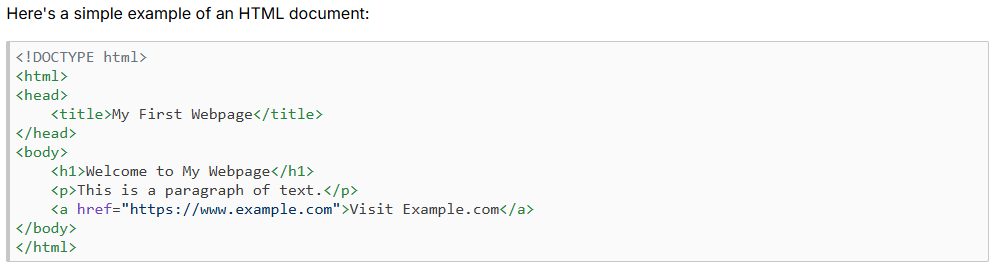
\includegraphics[width=\columnwidth]{figures/webdev-moodle.png}
\caption[WebDev lecture notes in Moodle]{An HTML example from the converted WebDev lecture notes in Moodle. Code is escaped and highlighted, so the example's tags appear as code.}
\label{fig:webdev_result}
\end{figure}

\subsection{Golden Tests}
\label{sec:ev_golden}

Whether a conversion is correct mostly depends on how the package looks in a player, which a unit
test cannot check.
Moreover, a chapter is a large JSON document, and after a change to the renderer the relevant
question is usually whether anything else changed, not whether a single field has a certain value.
The converter is therefore tested with \emph{golden cases}.
Each case is a small folder of Markdown files with a description of how to convert it.
The generated output, that is, the chapter JSON, the package metadata, the warnings, and the packed
images, is committed to version control next to it.
Running the tests writes the output of every case again, so the diff in version control is the
test result.
There is no comparison of expected and actual values and no pass or fail.
Every change in the output has to be reviewed, and if it is intended, it is committed together with
the change to the code.
For this comparison to be useful, the same input must always produce the same output.
Since every block carries a randomly generated identifier, all random values are taken from a single
source that returns a fixed sequence during the tests.
The corpus currently contains 128 cases covering every part of the conversion and merge.

\subsection{Conversion Time}
\label{sec:ev_time}

To determine how long a conversion takes, measurements were conducted on the 12-chapter WebDev corpus and each of the 128 golden cases separately.
They were taken on an AMD Ryzen 7 2700X with 32 GiB of RAM, running Windows 11 Pro and
Oracle Java 19.0.1.
For the warm-JVM measurements, every input was processed three times before ten recorded repetitions.
For comparison, a further ten CLI runs each started a new JVM\@.

\autoref{tab:conversion_time} reports means and sample standard deviations.
A complete conversion includes reading the local input, parsing, rendering, serializing the content,
and creating the package with its bundled libraries.
The parsing and rendering call was also measured separately on the same input.
An additional run measured the consecutive stages of conversion to identify the source of the
time difference.
The fresh CLI runs additionally include JVM startup and delivery of the output file.

\begin{table}[htbp]
\centering
\begin{tabular}{@{}lr@{}}
\toprule
Measurement & Time in ms, mean $\pm$ SD \\
\midrule
WebDev, complete conversion, warm JVM & $375.0 \pm 13.6$ \\
WebDev, parsing and rendering & $33.6 \pm 3.2$ \\
WebDev, packaging alone & $324.0 \pm 14.8$ \\
WebDev, fresh CLI process & $1801.3 \pm 22.2$ \\
\bottomrule
\end{tabular}
\caption[Conversion times for the WebDev lecture notes]{Conversion times for the WebDev lecture notes, with ten recorded repetitions per measurement.}
\label{tab:conversion_time}
\end{table}

The book can be regenerated in under two seconds on this machine, including JVM startup.
Most of the difference between parsing and rendering and a complete conversion comes from
packaging, which takes about 324 ms on its own.
Every conversion includes the same H5P libraries, even for a book containing only a few paragraphs.
For these inputs, packaging overshadows the differences in parsing and rendering.
The content's length and complexity therefore have only a small effect on total conversion time.

The golden cases were also timed individually to identify relatively expensive inputs.
Their mean complete conversion times range from 301 to 341 ms.
The much smaller parsing and rendering times in \autoref{tab:golden_time} again show how strongly the
common packaging work affects this comparison.
The \code{kitchen-sink} case, which comprises all the converter's supported features, takes the longest to parse and render, followed by several
image cases.

\begin{table}[H]
\centering
\small
\begin{tabular}{@{}lrr@{}}
\toprule
Golden Case & Parsing and Rendering & Complete Conversion \\
 & \multicolumn{2}{c}{Time in ms, mean $\pm$ SD} \\
\midrule
\code{kitchen-sink} & $8.3 \pm 1.3$ & $322.8 \pm 14.6$ \\
\code{image-paths} & $5.8 \pm 0.7$ & $311.5 \pm 11.4$ \\
\code{image-data-uri} & $4.3 \pm 0.5$ & $316.1 \pm 12.0$ \\
\code{image-shared-across-chapters} & $3.8 \pm 0.7$ & $309.3 \pm 10.8$ \\
\code{link-md-crosschapter} & $3.6 \pm 0.5$ & $318.4 \pm 30.5$ \\
\bottomrule
\end{tabular}
\caption[Golden cases with the longest parsing and rendering times]{The five golden cases with the longest mean parsing and rendering times, with ten recorded repetitions each.}
\label{tab:golden_time}
\end{table}

The 22 merge cases additionally measured merging after conversion.
Their mean merge times range from 324 to 360 ms; the combined \code{merge-kitchen-sink} case
requires $338.1 \pm 19.4$ ms.
This time includes reading both packages, alignment, and rewriting the output archive.
